% ==================================================================
% ch02 -- from the research note "Learning to Play"
% ==================================================================
\chapter{Learning to Play}
\label{ch:gam}

\noindent
A framework that explains everything after the fact explains nothing. The
previous chapter is a construction with a great many moving parts, and the
honest test of it is whether the parts pay for themselves on a domain where
we already know every answer and cannot be fooled about whether an
explanation is doing work.

So this chapter plays noughts-and-crosses. The whole game --- all 255{,}168
plays, all 5{,}478 reachable positions --- is small enough to enumerate
exactly, which means every claim below is a computed number rather than an
argument. A ladder of six theories is built inside the generated logic,
from ``take the centre'' to the exact minimax strategy, each rung priced by
the depth of the formula it installs, and each rung's winnings measured
against the metering.

Two results are worth knowing before the details arrive. The first is that
the logic dictates the encoding rather than the other way round: requiring
the notion of a fork to be expressible forces the board to be represented
with squares rather than lines as its components, and there is no freedom
in the matter. The second is that the true theory loses. The exact strategy
wins more games than any rung below it and is still the worst purchase on
the ladder, because it costs nearly three times what the rung below costs to
buy four percentage points. Truth here buys safety --- it is the only
strategy that never loses --- and safety is not food.

The chapter closes on a result i did not expect and have not been able to
argue away: a population that has completely solved its environment draws
every game, harvests nothing, and starves. A solved science is a dead
ecology. Imperfection is load-bearing.

\bigskip

\section{Introduction}\label{gam:S1}

\subsection{Why a worked example, and why this one}\label{gam:S1.1}

The companion note \chSci asks what it would take for a computation to
do science, and answers in four parts: the environment of a computation is other
computations; the hypothesis language is not chosen but generated from the
presentation of the calculus; a hypothesis becomes an experiment by being
installed as a guard, so that confirmation is a rendezvous; and the motive is
metabolic, since tokens are conserved, never minted, and a learner that predicts
badly starves.

Its Appendix A gives a small ecosystem in which every one of those constructions
appears as ordinary code. What that appendix does not do---and the omission is
the reason for this note---is show the framework \emph{reasoning}. Its
hypotheses are \texttt{q => q > 0} and \texttt{q => q > 4}: arithmetic
predicates on the size of a quantum. No formula in it uses a structural
connective, no assay discriminates between two structurally distinct
hypotheses, the relaxation lattice is never walked with anything on it, and at
no point does a better hypothesis visibly buy better performance. The appendix
demonstrates that the framework \emph{hosts} a learner. It does not demonstrate
that it \emph{produces} one.

The remedy is to instantiate the framework on a domain where the reader holds
the correct answers independently, so that what the machinery emits can be
scored against a standard the machinery did not supply. We take
noughts-and-crosses. The choice needs a defence, since the game is trivial, and
the defence is that triviality is the point: a worked example is for legibility,
not difficulty, and a game small enough to solve exhaustively is a game in which
every claim below can be checked rather than asserted. We checked all of them;
\S\ref{gam:sec:measure} reports the numbers and Appendix \ref{gam:app:repro} says how to
regenerate them.

\begin{remark}[The magic square comes free]\label{gam:magic-square-comes-free}
The obvious alternative---a magic-square puzzle---is the same problem. In the
game of \emph{Fifteen}, two players alternately claim numbers from $1$ to $9$
and the first to hold three summing to fifteen wins. Writing the numbers into a
Lo Shu square makes the triples summing to fifteen exactly the lines of a
three-by-three grid, and the two games are isomorphic. We mention this because
the puzzle framing is the one that would have been chosen for a solitary
solver, and the isomorphism shows what that framing costs: it hides the
opponent. An adversary is not an inconvenience here. It is the thing that makes
the environment a computation with a strategy to be learned, which is the only
kind of environment the companion note's ontology has.
\end{remark}

\subsection{What the mapping is supposed to show}\label{gam:S1.2}

Four features of the framework are exercised, and the interest is that each is
\emph{forced} by the domain rather than imposed on it.

\begin{description}
\item[A move is an assay.] One cannot observe an opponent without playing, and
  the position afterwards is not the position before. \S1.1 of \chSci
  argues that observation is action; here it is not an argument but the rules of
  the game.
\item[Minimax is an alternating modal formula.] The modalities are labelled by
  redex positions, and \S\ref{gam:sec:K} shows that in this domain a redex position
  \emph{is} a move. So $\exists s.\langle K_s\rangle \forall t. [K_t]\cdots$
  reads ``I have a move such that for every reply I have a move
  such that\ldots'', which is minimax written out, and the quantifiers range
  over something rather than standing in for it. Proposition~\ref{sci:prop:asymmetry} of
  \chSci then has something to say about which half of the game is
  cheap to learn.
\item[A fork is a separating conjunction.] Two threats whose completing squares
  are distinct. Disjointness is the entire content of the concept, and graded
  separation at $k=0$ is exactly disjointness of interface. \S\ref{gam:sec:board}
  shows that this demand dictates the board encoding.
\item[Destructive assay bites.] If winning harvests the loser, one never plays
  the same opponent twice, so hypotheses about individuals are worthless and the
  scientist must hold a hypothesis about a \emph{namespace} of opponents.
\end{description}

\subsection{What we are claiming, and what we are not}\label{gam:S1.3}

We claim that the framework, instantiated on this domain, generates a hypothesis
language in which the recognised concepts of the game are terms rather than
hand-coded features; that pricing those terms by modal depth produces a
cost--benefit structure with a measurable and non-obvious shape; and that three
of the companion note's propositions---the modal asymmetry, ``yield, not
truth'', and confinement---are visible in the measurements rather than merely
consistent with them.

We do not claim to have built a strong player. Noughts-and-crosses is solved and
a lookup table plays it perfectly; nothing here competes with that and nothing
should. Nor do we claim the pricing schedule is canonical: $\kappa(d)=2^{d}$ is
a choice, defended in \S\ref{gam:sec:price} and varied in \S\ref{gam:sec:measure}, and
the qualitative results survive the variation while the exact boundaries do not.
Finally, the guards below are written in the ideal logic. The current
interpreter accepts only the arithmetic and pattern fragment of the
\texttt{where} clause; where a guard uses a structural or modal connective it is
a specification of a check rather than a check the reducer performs, and we mark
each such occurrence.

\section{What this chapter carries forward}\label{gam:sec:import}\label{gam:S2}

Everything below is machinery from \chSci, restated compactly enough that the
worked example can be followed without turning back, and no more compactly than
that. Where a construction is used but not re-derived, the derivation is there;
the spatial--behavioural rubric is developed in~\cite{ClassifierNote}.

\paragraph{The cut, and three grades of access.} A world is $W \equiv S \mid E$:
the scientist and its environment, separated by parallel composition.
Computations are ontologically isolated, so $E$ is other computations, and what
$S$ can come to know of $E$ is bounded above by $E$'s context-labelled
bisimulation class. Access comes in exactly three grades: \emph{perception},
the structural predicates evaluated at the surface of $E$, priced by a schedule
$\kappa_{\mathrm{sense}}(d)$ monotone in formula depth; \emph{interaction}, the
context-labelled modalities, costing a rendezvous per step; and
\emph{reflection}, the name predicate $@\varphi$ applied to names $S$ already
holds, which is cheap because it passes through no surface.

\paragraph{The logic is generated.} Feeding the presentation of the \rh{}
calculus to the OSLF family yields one structural connective per term former,
one context-labelled modality per rewrite rule and redex position, and---because
$\mid$ carries an associative--commutative theory---a genuine separating
conjunction:
\[
P \models \varphi \mid \psi \iff P \equiv Q \mid R \text{ with } Q \models
\varphi,\ R \models \psi .
\]
Because a name is a quoted process, the name predicate $n \models @\varphi \iff
n = @P$ with $P \models \varphi$ sees into the structure of a name; this is
namespace logic \cite{NamespaceLogic}, in which one describes a namespace by a property
rather than enumerating it. The classifier note \cite{ClassifierNote} adds a
greatest fixed point $\nu X.\varphi$ and a \emph{graded separation} counting how
much of an interface two halves of a term share. We use both, but we take the
second in a form the next paragraph explains.

\paragraph{There is no restriction, so there is no hidden-name quantifier.}
The classifier note grades its separation over a vector of \emph{restricted}
names and reaches under the binder with a hidden-name quantifier $\Hq$. We do
not, because in this setting there is no binder. Restriction is syntactic sugar
(\chSci, Remark~\ref{sci:rem:sugar}): a name is a quoted process, and the calculus has a
standing theorem that no process ever contains the name that codes it.

\begin{proposition}[Freshness by quotation]\label{gam:prop:fresh}
Let $P$ be a process and $C[-]$ any context with $C[P] \neq P$. Then
$@C[P] \notin \mathrm{n}(P)$. Hence a name fresh in $P$ may be manufactured by
quoting any term properly containing $P$, with no registry and no consultation.
\end{proposition}
\begin{proof}[Proof sketch]
The no-self-code theorem gives $@Q \notin \mathrm{n}(Q)$ for every $Q$, and the
argument is a well-foundedness one: a name occurring in a term codes a strictly
smaller term. $C[P]$ properly contains $P$, so $@C[P]$ codes something larger
than $P$ and cannot occur among the names of $P$.
\end{proof}

Two things follow that the rest of the note uses. Freshness is
\emph{relative to a scope} rather than global, which is all any practical use
requires and which keeps the scheme decentralised---a central name server would
be an oracle sitting across the cut, contradicting isolation outright. And since
nothing is bound, nothing is hidden from description: $\Hq$ has no work to do,
and where the classifier note grades separation over a restriction vector we
grade it over a namespace given by a name predicate,
\[
P \models \varphi \mid_k^{N} \psi \iff P \equiv Q\mid R,\ \ Q \models \varphi,\
R \models \psi,\ \ |\,\mathrm{fn}(Q)\cap \mathrm{fn}(R) \cap N\,| = k ,
\]
with $N$ described rather than enumerated. Everything this note does that a
modal logic cannot do is done with $\mid_k^N$, and \S\ref{gam:sec:board} turns on
the choice of $N$.

\begin{remark}[Concealment is a price, not a wall]\label{gam:concealment-price-wall}
Removing restriction removes the only mechanism by which a computation could be
\emph{unobservable} rather than merely expensive to observe. That is not a loss;
it is the position \chSci already takes when it prices concealment by
a depth parameter $\delta$ instead of a barrier. It also settles a reading we
would otherwise have had to argue for: in \S\ref{gam:sec:world} we take $\delta$ to
be the number of plies of lookahead needed to model an opponent, and with no
restriction available that is the only thing $\delta$ \emph{can} be. A player's
strategy is never hidden. It is only ever deep.
\end{remark}

\paragraph{Hypotheses are guards.} The \texttt{where} clause of the \rh{}
calculus variant \cite{Omnibus} puts a formula in operational position:
$\texttt{for}(p \leftarrow c \ \texttt{where}\ \vartheta)P$. A hypothesis
installed as a guard is an experiment and a confirmation is a rendezvous;
nothing is carried and no interpreter is needed, and the cost of testing is
metered by the apparatus that meters everything else. An \emph{assay} is a
complementary guard pair, on $\varphi$ and on $\neg\varphi$, whose three
outcomes are \textsf{confirm}, \textsf{refute}, and $\bot$---the last being the
honest residue in which the environment did not answer in time.

\paragraph{The space and its metric.} Beneath the characteristic formula
$\chi_P$ sits a lattice of progressively weaker formulae obtained by forgetting
conjuncts. Hypotheses live there, and revision is a move on it. The metric is
ultrametric and stratified by the $\nu$-unfolding stage: $d(\varphi,\psi) =
2^{-n}$ when the two agree on all approximants below stage $n$ and differ at
$n$. Since modal depth is what a finite budget bounds, distance, depth, and cost
are one graded structure. The geometry is a tree, so there is no gradient, and
Proposition~\ref{sci:prop:confinement} of \chSci---\emph{confinement}---says a walk whose
steps are all shorter than $2^{-n}$ never leaves the ball of radius $2^{-n}$ it
started in.

\paragraph{The game.} Tokens are conserved: $\sigma + \kappa = \sigma_0 =
\Theta$, with $\sigma$ held in live stacks and $\kappa$ migrated into the
record. There is no primary producer. Under the internalising encoding
$\llbracket -\rrbracket : \Cost(\rh) \to \rh$ a located stack becomes a message
at a \emph{metabolic channel} $m_P$, and \emph{harvest} is an ordinary receipt
on $m_P$ performed by someone else. In $\Cost(\rh)$ stacks are inviolable; in
the image they are messages. The ecology lives in that gap, and Theorem~\ref{sci:thm:predator} of
\chSci identifies the predatory contexts as exactly the non-image
contexts holding a metabolic name. A \emph{game}, in the technical sense of
Definition~\ref{sci:def:game} there, is a choice of admitted context class $\mathcal{A}$ with
$\llbracket \Cost(\rh)\text{-Ctx}\rrbracket \subseteq \mathcal{A} \subseteq
\rh\text{-Ctx}$.

\section{The world}\label{gam:sec:world}\label{gam:S3}

\subsection{Three kinds of thing, and only one of them holds tokens}\label{gam:S3.1}

The world contains an \emph{arena}, a \emph{practice wall}, and a population of
\emph{players}.

The arena implements the rules. It alternates moves, detects completed lines,
and---this is the only thing about it that matters structurally---on a win it
hands the winner the loser's metabolic name. It holds no stack of its own and it
mints nothing. It \emph{routes}.

That distinction is what keeps \S16 of \chSci intact. The objection to
an exogenous reward signal is that it requires a referee holding a mint, and a
referee with a mint destroys conservation and with it the entire motivational
story. An arena that routes is not such a referee: every token it moves already
existed, in the loser's stack, and the total is unchanged. What the arena
supplies is not value but \emph{permission}.

\begin{observation}[The arena is the admitted context class]\label{gam:arena-admitted-context-class}
Definition~\ref{sci:def:game} of \chSci leaves $\mathcal{A}$ as a parameter and
observes that its two endpoints are degenerate: at one end the decorated
calculus with no game at all, at the other total war in which any context takes
anything it can address. A game of noughts-and-crosses picks out a specific
interior point. The contexts admitted to hold $m_P$ are exactly those that have
completed a line against $P$, and by Theorem~\ref{sci:thm:predator} those are non-image contexts. So
the rules of the game are not decoration on the ecology; the rules of the game
\emph{are} the choice of $\mathcal A$, and predation is legal here for precisely
one reason, which is that somebody won.
\end{observation}

\begin{remark}[Capability gating, concretely]\label{gam:capability-gating-concretely}
\chSci distinguishes the capability-gated game---contexts that
\emph{derive} $m_P$ from structure they can perceive---from one in which the
name is simply handed over. Noughts-and-crosses is gated in exactly that sense
once one asks how a player comes to complete a line: it must perceive the
position, and perceiving the position is priced. The derivation is the play.
\end{remark}

\subsection{The wall is a source, not a prey}\label{gam:S3.2}

A world in which the only food is other players is a world of pure
heterotrophs, and by \S11 of \chSci such worlds pay an unbounded
epistemic rent and are hard to keep alive. We therefore include a
\emph{practice wall}: a stationary player that moves uniformly at random, backed
by a finite reserve, which pays a small quantum per game played against it.

The wall has the access profile of a source in the precise sense of
\chSci, \S11.2: it is a persistent emitter, rate-limited by being a
single contract, non-exclusive since anyone may call it, non-adaptive because
its policy never revises, and exhaustible. A player is prey by the complementary
profile: a linear send, exhaustible, exclusive, and adaptive. The distinction is
not a difference of sort or of rewrite rule but of \emph{multiplicity}, which is
what makes the trophic split a fact about the cut rather than a taxonomy imposed
on it.

This gives the world its two order parameters in interpretable form.
\begin{itemize}
\item $\delta$, the concealment depth, is \emph{how many plies of lookahead are
needed to model one's opponent}. The wall has $\delta = 0$: its policy is
uniform and there is nothing to learn. A player running the top rung has a
$\delta$ of four or more.
\item $\iota$, the fraction of $\Theta$ already internal to scientists rather
than loose in the environment, is the ratio of the players' stacks to the wall's
remaining reserve. It rises monotonically as the wall is drained.
\end{itemize}

\subsection{Conservation, stated for this world}\label{gam:S3.3}

Write $\Theta = R_0 + \sum_i \sigma_i(0)$ for the wall's opening reserve plus
the players' opening stacks. Four operations move tokens and none creates them:
the wall's payout moves reserve into a player; harvest moves a loser's stack
into a winner's; endowment moves a parent's stack into a child's; and the
metabolic debit moves a token from $\sigma$ into $\kappa$. Hence $\sigma+\kappa
= \Theta$ at every step, and the world is a finite race. The listing of Appendix
\ref{gam:app:code} can be audited for this by inspection.

\section{The board: the logic dictates the encoding}\label{gam:sec:board}\label{gam:S4}

Here is the first place where the domain talks back, and we think it is the most
instructive moment in the note.

We want ``fork'' to be expressible, because a fork is the first genuinely
strategic concept in the game and because it is exactly the sort of thing a
game-playing program hand-codes as a feature. A fork is a double threat: a
position from which one has two distinct winning replies, so that the opponent
can block only one. Disjointness is the whole content: two threats sharing their
completing square are not a fork, they are one threat counted twice.

Separation is the connective for that. But which separation, and of what? The
answer depends on how the board is encoded, and the constraint turns out to be
tight.

\paragraph{The encoding.} A board $b$ carries, for each square $k$, two names
manufactured by reflection in the manner of the knot encoding's arcs: a
\emph{move channel} $\mathit{sq}_k = @[*b,k]$ and a \emph{mark cell}
$\mathit{mk}_k = @[*b,\texttt{"m"},k]$. These are not drawn from a stock of
atoms and they are not bound by anything. They are Proposition \ref{gam:prop:fresh}
in use: each is the quote of a term properly containing the board, hence fresh
in the board, and the family is generated by a decidable predicate on names, so
the whole namespace can be \emph{described}---which is what
$\mathit{Th}_b$ below does and what makes the graded separation available at
all. An empty square is a \emph{receipt} offering to be
claimed; an occupied square is the absence of that receipt together with a
resting send on its mark cell:
\[
\mathsf{Empty}_k \;\equiv\; \texttt{for}(@p \leftarrow \mathit{sq}_k\ \&\ @\_
\leftarrow \mathit{mk}_k)\{\ \mathit{mk}_k!(p)\ \}
\qquad\qquad
\mathsf{Held}_k(p) \;\equiv\; \mathit{mk}_k!(p) .
\]
In parallel sit eight \emph{line} processes. A line reads the three mark cells
of its line and replaces them; if it finds two marks of one player and one empty
square $s$, it deposits a standing \emph{offer} on a third family of names,
$\mathit{th}_s = @[*b,\texttt{"t"},s]$. A threat is therefore not computed on
demand. It is a piece of the term.

Offers live on their own names rather than on the move channels for a reason
worth stating: were a line to signal a threat by sending on $\mathit{sq}_s$, the
signal would rendezvous with the square's receipt and the line would have played
the move itself. Perception must not be able to act. That is the separation of
grades one and two of Table 1 of \chSci, enforced by the choice of
namespace.

\begin{definition}[Threat, fork]\label{gam:def:fork}
For a player $p$,
\[
\mathit{Th}_b := \{\, n : n \models @[*b,\texttt{"t"},\_\,] \,\}, \qquad
\Thr_s(p) := \lout(\mathit{th}_s)@p,
\]
\[
\Thr(p) := \exists s.\ \Thr_s(p) \mid \top,
\]
\[
\Frk(p) := \Thr(p) \mid_0^{\mathit{Th}_b} \Thr(p) .
\]
\end{definition}

$\mathit{Th}_b$ is the board's threat namespace, described by a name predicate
rather than listed. $\Frk(p)$ says the term splits into two parts, each carrying
an offer, \emph{sharing no name of that namespace}. Two threats at the same
square---two lines with a common gap---both deposit on $\mathit{th}_s$, so the
two parands share that name, $k \geq 1$, and $\mid_0^{\mathit{Th}_b}$ excludes
them. This is the graded separation of \cite{ClassifierNote}, \S2.3.2, used at the
bottom of its grading and graded over a described namespace rather than a
restriction vector; it was not introduced for this purpose.

\begin{figure}[t]
\centering
\fitwidth{%
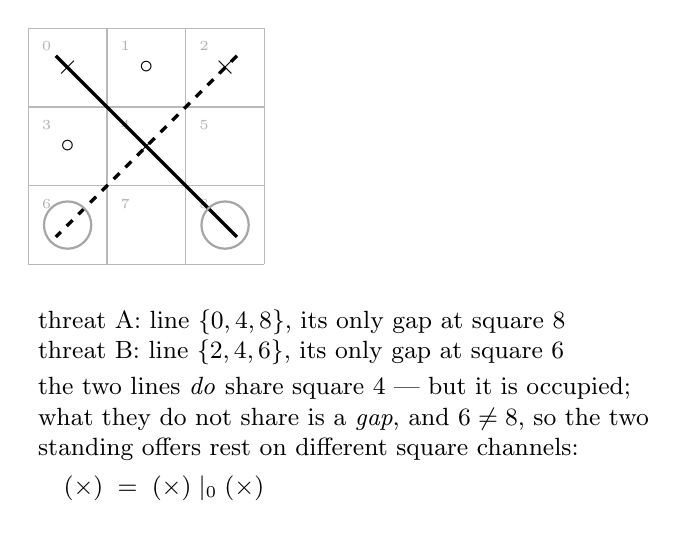
\begin{tikzpicture}[scale=1.0]
% grid
\foreach \i in {0,1,2,3} { \draw[gray!55] (\i,0) -- (\i,3); \draw[gray!55] (0,\i) -- (3,\i); }
% marks: X at 0,2,4 ; O at 1,3
\node at (0.5,2.5) {$\times$};  \node at (2.5,2.5) {$\times$};  \node at (1.5,1.5) {$\times$};
\node at (1.5,2.5) {$\circ$};   \node at (0.5,1.5) {$\circ$};
% square numbering, faint
\foreach \k/\x/\y in {0/0.5/2.5,1/1.5/2.5,2/2.5/2.5,3/0.5/1.5,4/1.5/1.5,5/2.5/1.5,6/0.5/0.5,7/1.5/0.5,8/2.5/0.5}
  {\node[gray!60,font=\tiny,anchor=north west] at (\x-0.45,\y+0.45) {\k};}
% the two threat lines
\draw[very thick] (0.35,2.65) -- (2.65,0.35);
\draw[very thick,dashed] (2.65,2.65) -- (0.35,0.35);
% the two gaps
\draw[thick,gray!70] (0.5,0.5) circle (0.3);
\draw[thick,gray!70] (2.5,0.5) circle (0.3);
% legend below
\node[anchor=north west,align=left,font=\small] at (0,-0.45)
 {threat A: line $\{0,4,8\}$, its only gap at square $8$\\
  threat B: line $\{2,4,6\}$, its only gap at square $6$\\[2pt]
  the two lines \emph{do} share square $4$ --- but it is occupied;\\
  what they do not share is a \emph{gap}, and $6 \neq 8$, so the two\\
  standing offers rest on different square channels:\\[3pt]
  \quad $\Frk(\times) \;=\; \Thr(\times) \mid_0 \Thr(\times)$};
\end{tikzpicture}}
\caption{A realised fork for crosses, and why $\mid_0$ at $k=0$ is the right
connective. Crosses threatens to complete on square $6$ or square $8$; noughts
can block only one. What the separation must exclude is a pair of threats with a
\emph{common} gap, since one move blocks both---and that is exactly what $k=0$
excludes once the squares, rather than the lines, are the parands
(Proposition~\ref{gam:prop:parands}).}
\label{gam:fig:fork}
\end{figure}

\begin{proposition}[The grading namespace must be indexed by square]\label{gam:prop:parands}
Let $\llbracket B \rrbracket$ be an encoding under which $\Frk(p)$ as given in
Definition \ref{gam:def:fork} is satisfied exactly by the positions in which $p$ has
a fork. Then the namespace $N$ over which $\mid_0^N$ counts sharing must be
indexed by the completing square, not by the line.
\end{proposition}
\begin{proof}[Proof sketch]
Two lines of a three-by-three grid meet in at most one square, so distinct lines
carry distinct line names and share none. Under a line-indexed encoding $\mid_0$
is therefore satisfied by any two distinct threats---including a pair whose gaps
coincide, for instance the two diagonals when only the centre is empty. That is
not a fork, since one move blocks both. Under the square-indexed encoding two
threats share a name iff they share their completing square, so $k=0$ holds iff
the gaps are distinct, which is the definition of a fork.
\end{proof}

\begin{remark}[What just happened]\label{gam:what-just-happened}
We did not choose the encoding and then ask what the logic could say about it.
We asked for a concept, and the requirement that the generated logic express it
determined the encoding. This is worth flagging because it is the mode in which
the framework is meant to be used and it is the opposite of the usual order. In
a hand-built game player, ``fork'' is a feature the programmer writes because
they know the game; here it is a formula in a logic nobody designed, and the
price of admission is a constraint on how the world is laid out. The companion
note argues that a generated logic is the right hypothesis language on grounds
of adequacy. This is the same claim cashed out as a design discipline.
\end{remark}

\subsection{The redex context is the move}\label{gam:sec:K}\label{gam:S4.1}

The modalities of the generated logic are labelled by contexts: one primitive
$\langle K_j\rangle$ per rewrite rule \emph{and choice of redex position}, where
$K_j$ is the one-hole context determined by that position
(\cite{ClassifierNote}, \S2.1). The label is not an action name. It records the
surroundings in which the step fires, and in this domain those surroundings are
exactly what carries the content.

The rho calculus has one interaction rule, so all the information in a label is
in the position. Write a world in play as
\[
W \;\equiv\; \Big(\ \prod_{k \in \mathrm{empty}} \mathsf{Empty}_k
\ \Big|\ \prod_{k \notin \mathrm{empty}} \mathsf{Held}_k(m_k)
\ \Big|\ L \ \Big|\ \mathit{Th} \ \Big|\ M_p \ \Big),
\]
with $L$ the line processes, $\mathit{Th}$ the standing offers, and $M_p$ the
mover's code, which for a move at $s$ contains the send $\mathit{sq}_s!(p)$.

\begin{definition}[The move context]\label{gam:def:K}
For an empty square $s$, the redex position of the claim at $s$ is the join of
$\mathit{sq}_s!(p)$ with $\mathsf{Empty}_s$, and the one-hole context
determined by it is
\[
K_s \;:=\; \Big(\ [\,\cdot\,]\ \Big|
\prod_{k \in \mathrm{empty},\ k \neq s}\!\! \mathsf{Empty}_k \ \Big|
\prod_{k \notin \mathrm{empty}}\!\! \mathsf{Held}_k(m_k) \ \Big| \ L \ \Big|\
\mathit{Th} \ \Big| \ M_p' \Big) ,
\]
$M_p'$ being the mover's remaining code. We write $\langle K_s\rangle\varphi$
for the corresponding generated modality.
\end{definition}

\begin{proposition}[Moves are redex positions]\label{gam:prop:moves}
The redex positions of $W$ at which a claim can fire are in bijection with the
empty squares, and the mover is determined by the context. Hence
\[
\text{``$p$ has a move $s$ after which $\varphi$''}
\quad=\quad
\exists s.\ \langle K_s \rangle \varphi ,
\]
where the existential ranges over redex positions, and the branching factor of
that quantification is the number of legal moves.
\end{proposition}
\begin{proof}[Proof sketch]
An occupied square offers no receipt, so no claim can fire there; each empty
square offers exactly one, and the mark cells are disjoint, so the receipts do
not race with each other. Distinct $s$ give distinct contexts, since $K_s$
retains $\mathsf{Empty}_{s'}$ for every $s' \neq s$ and $K_{s'}$ does not.
Whose move it is, is fixed by which $M_p$ sits in the context.
\end{proof}

\begin{remark}[Why an action label would not do]\label{gam:why-action-label-would}
Every claim, at every square, by either player, is the same action: a comm on a
square channel carrying a mark. An action-labelled modal logic in the style of
Hennessy--Milner sees one label and cannot distinguish nine moves; recovering
the distinction would mean encoding the square into a name discipline and then
reasoning about names, which is the manoeuvre \cite{ClassifierNote}, \S3.1 declines
in the knot setting for the same reason. Context-labelling gives it directly:
the square being claimed is the hole, and everything else is the label.
\end{remark}

\begin{lemma}[The board settles]\label{gam:lem:settle}
After a claim fires, the line processes run to a unique normal form in finitely
many steps, and the resulting family of offers depends only on the marks.
\end{lemma}
\begin{proof}[Proof sketch]
Each of the eight lines performs one join on three mark cells and replaces what
it took, so no line's output enables another: offers are deposited on the
$\mathit{th}$ names, which no line reads. The settling is therefore a finite,
conflict-free sequence of eight steps up to the ordinary races for mark cells,
and those commute because each restores its cell unchanged. Hence confluence and
termination.
\end{proof}

\begin{definition}[The settled modality]\label{gam:settled-modality}
$\langle\!\langle K_s \rangle\!\rangle \varphi$ holds when the claim at $s$
fires and $\varphi$ holds of the term after the settling of Lemma
\ref{gam:lem:settle}. This is the weak diamond, and Lemma \ref{gam:lem:settle} makes it
deterministic in $s$.
\end{definition}

We use $\langle\!\langle - \rangle\!\rangle$ throughout, and note that a plain
$\langle K_s\rangle$ would land the scientist between a move and the world's
recognition of it---a state in which the threat structure is stale. That the
distinction has to be drawn at all is a fact about a world in which perception
is a process rather than a lookup.

\section{The ladder}\label{gam:sec:ladder}\label{gam:S5}

\subsection{Six rungs and a limit}\label{gam:S5.1}

The relaxation lattice for this domain has a ladder through it that every human
learner of the game climbs, and it is convenient that the ladder is already
named: it is essentially Newell and Simon's rule list. We write it in the
generated logic, cumulatively, each rung adding one disjunct above the previous
ones in priority.

\begin{center}
\fitwidth{%
\begin{tabular}{@{}cll@{}}
\toprule
rung & formula added & kind and depth \\
\midrule
0 & $\top$ & --- \\[3pt]
1 & $\exists s.\ \mathsf{Emp}(s) \wedge \Thr_s(\text{me})$
  & spatial, depth 1 \\[3pt]
2 & $\exists s.\ \mathsf{Emp}(s) \wedge \Thr_s(\text{them})$
  & spatial, depth 1 \\[3pt]
3 & $\exists s.\ \langle\!\langle K_s\rangle\!\rangle \Frk(\text{me})$
  & one modal step over $\mid_0$ \\[3pt]
4 & $\exists s.\ \forall t.\ \langle\!\langle K_s\rangle\!\rangle
    [\![K_t]\!]\, \neg\Frk(\text{them})$
  & box under diamond, depth 2 \\[3pt]
5 & $\Ctr$ & name-level, depth 0 \\[3pt]
6 & $\chi := \nu X.\ \forall s.\, [\![K_s]\!]\big(\neg\mathsf{Lost} \wedge
    \exists t.\ \langle\!\langle K_t\rangle\!\rangle X\big)$
  & full alternation \\
\bottomrule
\end{tabular}}
\end{center}

Here $\mathsf{Emp}(s) := \lin(\mathit{sq}_s)\top$---the square still offers a
receipt, a structural predicate of depth one---and $\Ctr$ is a preference over
square \emph{names}, read off the reflected structure $@[*b,k]$ by a name
predicate, containing no modality and requiring no step at all. The quantifiers
$\exists s$ and $\forall t$ range over redex positions, which by Proposition
\ref{gam:prop:moves} is to say over legal moves.

Two features of the shape are worth naming, and both were invisible while $K$
was an uninstantiated placeholder.

\begin{observation}[Winning and blocking are perception, not lookahead]\label{gam:winning-blocking-perception-lookahead}
Rungs 1 and 2 contain no modality. Having a winning move is not a fact about
what would happen if one moved; it is the fact that a completing offer stands at
a square still open, and the line processes deposited that offer when the world
last settled. The scientist reads it. The behavioural content was pushed into
the structure of the term by a computation somebody else already paid for.
\end{observation}

This has a general form, and it is the most useful thing in the section. There
are two routes to any predicate about the environment: \emph{read} it, if the
environment has already computed it into legible structure, or \emph{drive} it,
by taking steps and watching. The first is perception and the second
interaction---grades one and two of Table 1 of \chSci---and they are
priced by different schedules, one by formula depth and one by rendezvous. An
environment that computes a great deal about itself into structure is one in
which a poor scientist can nonetheless know much; an environment that computes
nothing until driven is one where knowledge is available only to those who can
afford to act. That is a claim about environments rather than about learners,
and this framework can state it because it prices the two grades separately.

\begin{observation}[The asymmetry has moved to the right place]\label{gam:obs:asym}
With $K$ instantiated, the existential and universal quantifiers range over
moves, and the ladder's one genuinely alternating rung is rung 4:
$\exists s \forall t$, a box under a diamond. By Proposition~\ref{sci:prop:asymmetry} of
\chSci the diamond has a finite confirming witness and the box has
none, so rung 4 is the rung whose confirmation is unbounded and whose refutation
is cheap. Section \ref{gam:sec:measure} finds that it is also, by a wide margin, the
worst purchase on the ladder: $+0.005$ of win probability for $111$ metered
units. Making a fork is establishing an existential; preventing one is
discharging a universal, and the framework prices that difference before
measuring it.
\end{observation}

\begin{remark}[Why $\chi$ is reachable here, and what that costs later]\label{gam:why-reachable-here-what}
Proposition~\ref{sci:prop:limit} of \chSci says the complete theory of an environment is
unaffordable when its recursion follows the reduction rather than a finite
structural cycle. Noughts-and-crosses is the converse case of Remark~\ref{sci:rem:structural} there:
the board loses a square at every step, so the alternation in $\chi$ bottoms out
and $\nu$ is exact at a finite unfolding---nine, in fact. This is a \emph{closed}
science, one of the subject matters admitting a complete finite theory. That is
what makes the domain a good demonstration and, as \S\ref{gam:sec:death} shows, what
kills the ecology.
\end{remark}

\subsection{The rungs are the $\nu$-approximants}\label{gam:S5.2}

The ladder is not merely ordered; it is metrically graded, and by the metric the
companion note already fixed.

\begin{proposition}[The ladder is a chain of shrinking steps]\label{gam:ladder-chain-shrinking-steps}
Under the stratified distance of \chSci, Definition~\ref{sci:stratified-distance}, the rungs
agree on every approximant below the stage at which the added conjunct first
looks and differ at that stage. Rungs 1 and 2 add conjuncts that inspect the
settled term without stepping, and so sit at stage 1; rung 3 adds one
$\langle\!\langle K_s \rangle\!\rangle$, reaching stage 2; rung 4 adds a box
beneath it, reaching stage 3; and $\chi$ is the limit of the sequence. Hence
$d(\varphi_r,\varphi_{r+1}) = 2^{-r}$ for $r = 1, \dots, 4$, and the steps
shrink as one climbs.
\end{proposition}

Two consequences follow immediately and they are the ones that structure
\S\ref{gam:sec:confine}. First, moving from rung $r$ to rung $r+1$ is a \emph{short}
move---distance $2^{-r}$, shrinking as one deepens---so by confinement a
scientist that only ever deepens can never leave the ball its early commitments
placed it in. Second, by Proposition~\ref{sci:prop:movecost} of \chSci, cost is monotone in
distance, so the cheap moves are exactly the confined ones.

\subsection{The modal asymmetry, and what it predicts}\label{gam:S5.3}

Observation \ref{gam:obs:asym} located the ladder's one alternating rung. It is
worth writing the asymmetry out, now that the quantifiers have something to
range over:
\[
\underbrace{\exists s.\ \langle\!\langle K_s\rangle\!\rangle \Frk(\text{me})}
_{\text{a finite witness: exhibit the square}}
\qquad\text{versus}\qquad
\underbrace{\exists s.\ \forall t.\ \langle\!\langle K_s\rangle\!\rangle
[\![K_t]\!]\,\neg\Frk(\text{them})}
_{\text{no finite witness: every reply must be checked}} .
\]
Establishing that one \emph{can} fork requires producing the move. Establishing
that a move is \emph{safe} requires discharging a universal over the opponent's
replies, and by Proposition~\ref{sci:prop:asymmetry} of \chSci no finite run witnesses that;
only a counterexample is finite. The framework therefore predicts, from the
shape of the formula rather than from anything about games, that offensive
knowledge is the cheaper acquisition---which is what every human learner of the
game in fact does, and which \S\ref{gam:sec:measure} confirms in the currency that
matters here: rung 4 is the worst purchase on the ladder.

There is a second, independent measurement of the same asymmetry. Restricting
the top heuristic rung to each colour separately: as the first player it
achieves the game-theoretic value against a perfect opponent, drawing every
game; as the second player it loses $6.3\%$. The same policy is complete on
offence and incomplete on defence.

\begin{remark}[A reading, offered as such]\label{gam:reading-offered-as-such}
We resist over-claiming on the second measurement. The first player has the
initiative, so existential reasoning is more nearly sufficient for it, and one
could attribute the colour asymmetry to that alone. What the framework adds is a
reason the two are not symmetric \emph{in price}: the universal formula is the
one whose confirmation has no finite witness, so a budget-bounded learner
confirms attacks and can only ever refute claims of safety. We take the colour
measurement as consistent with Proposition~\ref{sci:prop:asymmetry}; the rung-4 cost is the
demonstration.
\end{remark}

\section{The assay}\label{gam:sec:assay}\label{gam:S6}

A move is an experiment, and in this domain that is not a metaphor to be
maintained but the only thing a move can be.

\begin{definition}[The move-assay]\label{gam:move-assay}
For a scientist holding hypothesis $\varphi$ with metabolic channel $m$,
a move on probe channel $p$ is
\begin{center}
\begin{minipage}{0.9\textwidth}
\begin{lstlisting}
contract Move(b, @hyp, @me, ret) = {
  new probe in {
      @[*b, "offer"]!(*probe, me)            // the probe perturbs the world
    | for (@pos <- probe where pos |= hyp)    { ret!(("confirm", pos)) }
    | for (@pos <- probe where ~(pos |= hyp)) { ret!(("refute",  pos)) }
  }
}
\end{lstlisting}
\end{minipage}
\end{center}
\end{definition}

The complementary pair is what makes this more than an expression of hope: in a
concurrent setting a guard that simply fails to fire cannot be distinguished
from a guard still waiting, so the negated guard is what separates refutation
from patience. The three outcomes of Proposition~\ref{sci:prop:trichotomy} of \chSci are
three code paths, one of which is empty---and in this domain the empty path has
a concrete reading. If the opponent does not reply within the budget, the game
is abandoned unresolved; the scientist learns nothing and has paid for the
attempt. That is $\bot$, and it is neither confirmation nor refutation.

\begin{remark}[Where the checker is]\label{gam:where-checker}
Nothing in the listing consults a hypothesis and then decides. The hypothesis is
in guard position, so the reduction rule is the checker, and the cost of testing
is metered by the same apparatus that meters the move. An unpriced test would be
an oracle and would collapse the motivational story entirely; this is the
concrete form of that constraint.
\end{remark}

\subsection{Pricing}\label{gam:sec:price}\label{gam:S6.1}

We charge each rule the depth of the formula it installs, times the number of
candidate moves it must examine:
\[
\kappa(d) = 2^{d}, \qquad
\text{cost of a decision at rung } r \;=\; |M| \cdot \!\!\sum_{\text{rules } 1..r}\!\! \kappa(d_{\text{rule}}) ,
\]
with $|M|$ the number of legal moves---which by Proposition \ref{gam:prop:moves} is
the branching factor of the quantification over redex positions, so the two
readings of $|M|$ agree. Rungs 1 and 2, being structural at depth 1, cost $2$
per candidate each; rung 3 adds $4$ for its single settled step over a
separation; rung 4 adds $8$ for the box beneath the diamond; $\Ctr$, being
name-level at depth 0, adds $1$; and $\chi$ costs $32$.

Three comments. The schedule is a \emph{choice}, and \S\ref{gam:sec:measure} varies
it. The exponential shape is not arbitrary: it is what makes distance, depth,
and cost one graded structure, which is the reason \chSci prefers the
$\nu$-stratified ultrametric to a measure-theoretic alternative. And the
positional rung costing almost nothing is not a thumb on the scale; it is a
consequence of $\Ctr$ containing no modality, hence requiring no lookahead. That
this cheap rung turns out to be the most profitable one on the ladder is the
main empirical finding below, and it would have been invisible under a schedule
that priced by rung index rather than by formula depth.

\section{Destructive assay, again}\label{gam:sec:destructive}\label{gam:S7}

Section 8 of \chSci argues that because harvest ends the prey's
computational life, each specimen affords exactly one measurement, so hypotheses
about individuals are worthless and the hypothesis language must be a logic of
namespaces. The argument is abstract there. Here it is the situation.

A scientist that wins eats its opponent, so it never faces that opponent again.
It cannot accumulate a model of \emph{this} player across games; what it can
accumulate is a model of the \emph{kind} of player---a namespace description,
satisfied by many opponents, and the thing a name predicate $@\varphi$ states.
Every rung of \S\ref{gam:sec:ladder} is of this form: none of them mentions an
individual, all of them describe a class of positions or a class of policies.

There is a corollary worth making explicit because it has a familiar shape.

\begin{proposition}[Learning requires a population]\label{gam:learning-requires-population}
In a world where victory is fatal to the loser, no single scientist can test a
hypothesis about opponent policy more than once against the same opponent.
Statistical confirmation therefore requires either many opponents drawn from one
namespace, or a lineage that inherits the hypothesis. The wall supplies the
first and \S\ref{gam:sec:confine} supplies the second.
\end{proposition}

This is the same conclusion \S17.2 of \chSci reaches for continual
learning by a different route: a population is required rather than merely
preferred.

\section{The measurements}\label{gam:sec:measure}\label{gam:S8}

Everything in this section is exact rather than sampled. The game has $5{,}478$
reachable positions, $765$ up to the symmetries of the square, and $255{,}168$
distinct plays; of its $4{,}520$ non-terminal positions, $1{,}890$---$41.8\%$---
offer a fork to the player to move, which is why the rung-3 conjunct is worth
having at all. Outcome distributions and expected metering are computed by
recursion over the whole tree, with ties within a rung broken uniformly.
Figures below are symmetrised over colour: each policy plays first half the
time.

\subsection{The ladder pays, and where}\label{gam:S8.1}

\begin{table}[h]
\centering
\fitwidth{%
\begin{tabular}{@{}clrrrrrr@{}}
\toprule
rung & added conjunct & win & draw & loss & cost & $\Delta$win & return \\
\midrule
0 & $\top$                                  & 0.437 & 0.127 & 0.437 & 0.0 & --- & --- \\
1 & $\Thr_s(\text{me})$                     & 0.668 & 0.075 & 0.258 & 40.9 & $+0.231$ & $+0.0057$ \\
2 & $\Thr_s(\text{them})$                   & 0.798 & 0.165 & 0.037 & 77.8 & $+0.130$ & $+0.0035$ \\
3 & $\langle\!\langle K_s\rangle\!\rangle\Frk$ & 0.831 & 0.135 & 0.035 & 134.9 & $+0.033$ & $+0.0006$ \\
4 & $\forall t.[\![K_t]\!]\neg\Frk$         & 0.836 & 0.138 & 0.027 & 245.7 & $+0.005$ & $+0.00005$ \\
5 & $\Ctr$                                  & \textbf{0.918} & 0.080 & 0.002 & 255.9 & $+0.083$ & $\mathbf{+0.0082}$ \\
6 & $\chi$                                  & 0.873 & 0.127 & \textbf{0.000} & 679.2 & $-0.046$ & $-0.0001$ \\
\bottomrule
\end{tabular}}
\caption{The ladder against a uniform-random opponent. ``cost'' is expected
metering per game under $\kappa(d)=2^d$; ``return'' is $\Delta$win per metered
unit. Loss rate falls monotonically along the whole ladder. Win rate does not:
it peaks at rung 5.}
\label{gam:tab:ladder}
\end{table}

\begin{figure}[h]
\centering
\fitwidth{%
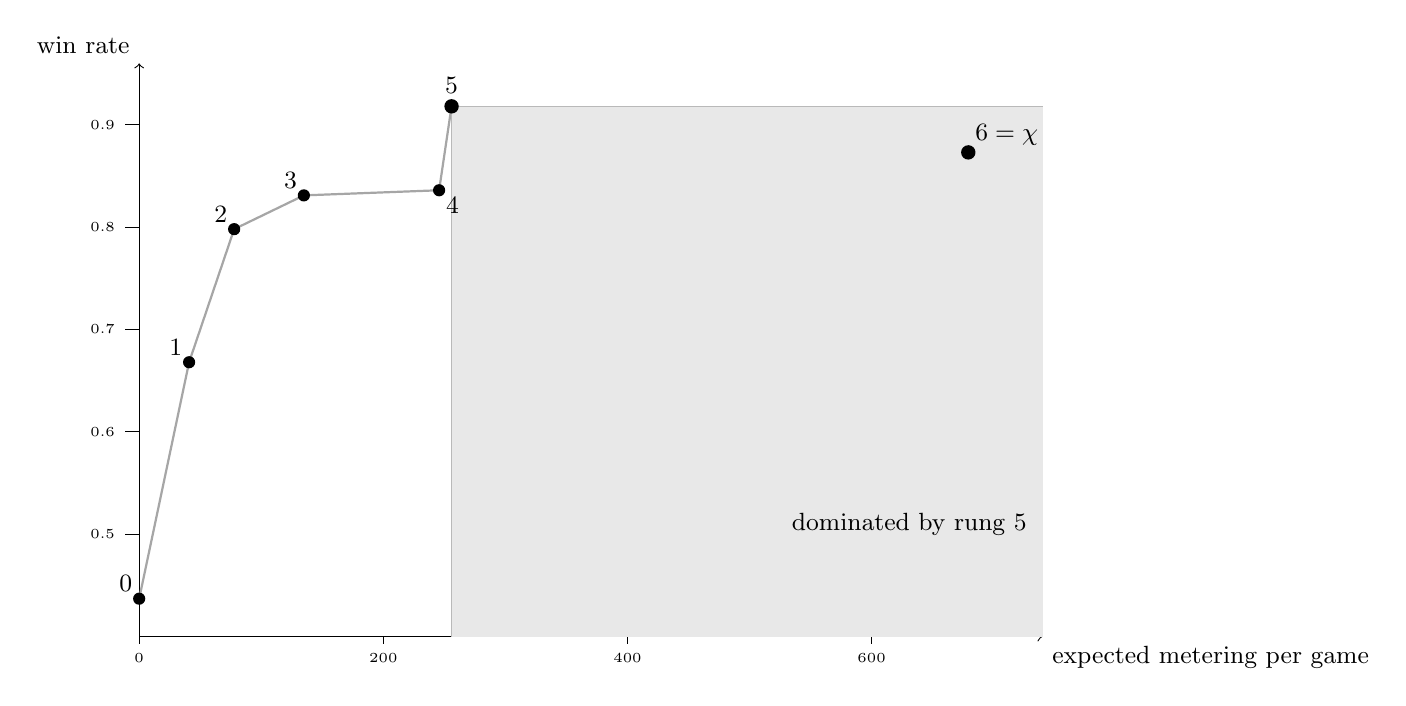
\begin{tikzpicture}[x=0.0155cm,y=13cm]
% axes
\draw[->] (0,0.40) -- (740,0.40) node[below right,font=\small] {expected metering per game};
\draw[->] (0,0.40) -- (0,0.96) node[above left,font=\small] {win rate};
\foreach \x in {0,200,400,600} \draw (\x,0.40) -- (\x,0.393) node[below,font=\tiny] {\x};
\foreach \y in {0.5,0.6,0.7,0.8,0.9} \draw (0,\y) -- (-12,\y) node[left,font=\tiny] {\y};
% ladder path
\draw[thick,gray!70] (0,0.437) -- (40.9,0.668) -- (77.8,0.798) -- (134.9,0.831) -- (245.7,0.836) -- (255.9,0.918);
\draw[thick,gray!70,dashed] (255.9,0.918) -- (679.2,0.873);
% dominated region for rung 5
\fill[gray!18] (255.9,0.40) rectangle (740,0.918);
\draw[gray!55] (255.9,0.918) -- (740,0.918);
\draw[gray!55] (255.9,0.40) -- (255.9,0.918);
% points
\foreach \x/\y/\l in {0/0.437/0,40.9/0.668/1,77.8/0.798/2,134.9/0.831/3}
  {\fill (\x,\y) circle (2.2pt); \node[font=\small,above left=-1pt] at (\x,\y) {\l};}
\fill (245.7,0.836) circle (2.2pt); \node[font=\small,below right=-1pt] at (245.7,0.836) {4};
\fill (255.9,0.918) circle (2.6pt); \node[font=\small,above=1pt] at (255.9,0.918) {5};
\fill (679.2,0.873) circle (2.6pt); \node[font=\small,above right=-1pt] at (679.2,0.873) {$6=\chi$};
\node[font=\small,anchor=north east] at (735,0.53) {dominated by rung 5};
\end{tikzpicture}}
\caption{The ladder as a cost--yield curve, against a uniform-random opponent.
Rungs 1--4 show sharply diminishing returns for a roughly doubling price, rung 4
---the alternating one---being the flattest. Rung 5, a predicate on square names
of depth zero, is nearly free and delivers the largest jump on the ladder. The complete theory $\chi$ lies inside the shaded
region: it costs more than rung 5 and wins less, so it is dominated on both
axes.}
\label{gam:fig:pareto}
\end{figure}

Three features of Table \ref{gam:tab:ladder} deserve separate statements.

\begin{observation}[Diminishing returns, until they don't]\label{gam:diminishing-returns-until-they}
Marginal return falls by more than two orders of magnitude from rung 1 to rung
4---$+0.0057$, $+0.0035$, $+0.0006$, $+0.00005$---while cost roughly doubles at
each step. Rung 4 in particular buys $+0.005$ of win probability for $111$
metered units, and it is the alternating rung of Observation \ref{gam:obs:asym}: the
one whose formula has no finite confirming witness. A budget-bounded learner
would stop before it, and the foraging
inequality of \chSci, Proposition~\ref{sci:prop:foraging}, says exactly when: harvest
credits the scientist only if the prey's stack exceeds what finding and opening
it cost.
\end{observation}

\begin{observation}[The non-modal rungs carry the ladder]\label{gam:obs:spatial}
Once $K$ is instantiated, three of the five useful rungs turn out to contain no
modality: rungs 1 and 2, which read standing offers, and rung 5, which reads
square names. Together they deliver $+0.444$ of the ladder's total $+0.481$ gain
---$92.3\%$ of the yield---for $87.9$ of its $255.9$ metered units, or $34.3\%$
of the cost. The two modal rungs deliver the remaining $+0.038$ for $168.0$
units. Rung 5 alone returns $+0.0082$ per unit, the best figure on the ladder
and some one hundred and sixty times rung 4's.
\end{observation}

This is the result we would lead with, and it is one we could not have stated
before the correction: with $\langle K\rangle$ standing in as a placeholder,
rungs 1 and 2 looked modal, and the split between reading and driving was
invisible. The classifier note argues, in the knot setting, that the spatial
layer is where the generated logic earns its name and that a purely behavioural
logic cannot state the properties that matter (\cite{ClassifierNote}, Remark 5).
That argument is made there on expressiveness grounds. Here it is cashed in an
ecological currency: the non-behavioural fragment is not merely
expressible-and-useful, it is where nearly all the yield per token lives, and a
mortal learner that priced its own hypotheses would find it first. A modal logic
could not have offered any of it.

\begin{remark}[Why this is not an artefact of the encoding]\label{gam:why-this-artefact-encoding}
One might object that we simply put the threats into the term, so of course
reading them is cheap. The objection has force and the answer is that somebody
paid: the line processes run on every settling, and \S\ref{gam:sec:price} charges
that scan. What the encoding does is \emph{relocate} the cost, from the
scientist's budget to the world's---and that relocation is precisely the
distinction between an environment one can perceive and one that must be driven.
The interesting quantity is not whether the work is done but who is billed for
it, which is a question this framework can pose because both parties have
stacks.
\end{remark}

\begin{observation}[The true theory is dominated]\label{gam:obs:chi}
$\chi$ is the complete theory: it never loses, from either colour, against any
opponent. It is also, against fallible prey, strictly worse than the heuristic
rung below it on both axes at once. Against a random opponent rung 5 wins
$0.918$ at cost $255.9$ while $\chi$ wins $0.873$ at cost $679.2$; against a
rung-4 opponent, $0.448$ at $280.3$ versus $0.418$ at $708.8$. Fewer wins, and
between one and a half and two and a half times the price.
\end{observation}

The mechanism is not mysterious and is well known to anyone who has implemented
game search: minimax assumes optimal opposition, so it settles for a draw in
positions where a heuristic would set a trap that a fallible opponent walks
into. What is worth noting is that the framework \emph{predicted} this before we
measured it. Remark~\ref{sci:rem:yieldbias} of \chSci says that a mortal scientist is not
rewarded for holding true hypotheses but for holding nutritive ones, and that a
lineage under selection drifts toward yield-biased search wherever yield and
discrimination disagree. Here they disagree, the disagreement is measurable, and
it runs in the predicted direction.

\begin{corollary}[Truth buys safety, not food]\label{gam:truth-buys-safety-food}
$\chi$ is the unique rung with loss probability zero. So the complete theory
does buy something the heuristic does not---it cannot be beaten---but what it
buys is insurance rather than yield. In a world where survival is the only score
and the prize is another's stack, insurance is worth having only when the stakes
are large enough to matter, which is the next calculation.
\end{corollary}

\subsection{Invasion, and the price of being right}\label{gam:S8.2}

Take a population fixed at rung 5 and ask when a $\chi$-holding mutant invades.
Head to head, $\chi$ wins $3.17\%$ and never loses; it costs $720.0$ per game
against the resident's $324.0$. The mutant is favoured when $\sigma \cdot
0.0317 > \text{price} \cdot 396.0$, that is when
\[
\sigma \;>\; 12474 \cdot \text{price},
\]
where $\sigma$ is the prey stack won and \emph{price} converts metered units
into tokens. The complete theory is therefore a luxury good, purchasable only
where the stakes are some twelve thousand times the unit cost of thought.

\begin{remark}[Basic research, priced]\label{gam:basic-research-priced}
Remark~\ref{sci:rem:pragmatist} of \chSci concedes the pragmatist's objection---this
scientist's epistemology is metabolic and truths that do not pay go
unfunded---and answers with surplus: a scientist holding more than its foraging
horizon requires can afford inquiry that does not pay. The number above is that
remark made quantitative for one domain. Truth is affordable here, and only
here, above a threshold; below it, the ecology selects for a theory that is
known to be wrong and known to be more profitable. Pricing the ladder by the
instantiated formulae rather than by rung index raises that threshold by a
factor of three, because the cheap rungs turn out to be cheaper than a
placeholder $\langle K\rangle$ made them look.
\end{remark}

\subsection{The phase band}\label{gam:S8.3}

Table \ref{gam:tab:phase} reports, for each opponent depth and each prey stack, which
rung maximises $\sigma\cdot P(\text{win}) - \text{price}\cdot \mathbb{E}[\text{cost}]$.

\begin{table}[h]
\centering
\fitwidth{%
\begin{tabular}{@{}rccccccc@{}}
\toprule
$\sigma$ & vs r0 & vs r1 & vs r2 & vs r3 & vs r4 & vs r5 & vs r6 \\
\midrule
20   & 2 & 2 & 0 & 0 & 0 & 0 & 0 \\
50   & 2 & 2 & 3 & 3 & 5 & 0 & 0 \\
100  & 5 & 5 & 5 & 5 & 5 & 0 & 0 \\
200  & 5 & 5 & 5 & 5 & 5 & 2 & 0 \\
400  & 5 & 5 & 5 & 5 & 5 & 2 & 0 \\
800  & 5 & 5 & 5 & 5 & 5 & 2 & 0 \\
1600 & 5 & 5 & \textbf{6} & \textbf{6} & 5 & 2 & 0 \\
\bottomrule
\end{tabular}}
\caption{Optimal rung, at price $0.05$ per metered unit, as a function of the
prey's stack $\sigma$ (rows) and the prey's own rung (columns). The optimal rung
is $0$ in both extremes and interior in between.}
\label{gam:tab:phase}
\end{table}

The shape is the phase diagram of \chSci, \S13.2, in a domain where
both order parameters have concrete readings.

\begin{itemize}
\item \textbf{Low $\delta$, low stakes: theory is overhead.} Against a shallow
opponent worth little, rung 0 or 1 is optimal. Reflex beats inquiry; a theory is
something one is paying to carry.
\item \textbf{High $\delta$: inquiry cannot pay.} Against a rung-6 opponent the
optimal rung is $0$ at \emph{every} stake, because no rung ever beats it, so the
cheapest available policy maximises net. This is the upper boundary, and it has
a bracing reading: against an environment one cannot model within any affordable
budget, the correct scientific policy is not to try.
\item \textbf{The band between.} For intermediate opponents and stakes, an
interior rung is optimal---mostly rung 5, the heuristic, not rung 6, the truth.
\end{itemize}

$\chi$ is optimal in exactly two cells of the whole grid, both at the cheapest
price and the largest stake. Raising the price to $0.2$ and to $1.0$ shifts the
band toward the cheap rungs without changing its shape: at price $1.0$ the
optimal rung is $0$ over most of the table and never $6$ anywhere. The
qualitative structure---interior optimum, degenerate at both ends---is robust;
the boundaries are not.

\section{Confinement, measured}\label{gam:sec:confine}\label{gam:S9}

This section is the one we would keep if we could keep only one, because it
turns Proposition~\ref{sci:prop:confinement} of \chSci from a fact about ultrametric spaces
into a fact about a hypothesis space someone might actually hold.

\subsection{Two loci, and only one of them is reachable}\label{gam:S9.1}

A policy on this ladder has exactly two parameters, and they are the two that
Definition~\ref{sci:def:move} of \chSci says a revision move must choose: a
\emph{locus} and an \emph{operation}. The loci here are

\begin{itemize}
\item the \textbf{opening}---which square to take first---which is the stage-1
approximant, at metric distance $2^{-1}$; and
\item the \textbf{rung}---how deep the theory runs---which is everything at
stage 2 and below.
\end{itemize}

Deepening the rung is a short move: from rung $r$ to rung $r+1$ is a step of
$2^{-r}$. Changing the opening is a long one. By confinement, a scientist whose
revisions are all deepenings can never change its opening, however long it lives
and however many refutations it suffers. In the listing of Appendix
\ref{gam:app:code} this is visible as a fact about the code: \texttt{Revise} only
ever increments the rung.

\subsection{The measurement}\label{gam:S9.2}

Lock the opening and let both sides otherwise play the top heuristic rung. Then
against a rung-2 opponent:

\begin{center}
\fitwidth{%
\begin{tabular}{@{}lrr@{}}
\toprule
opening & win rate at rung 5 & win rate at rung 6 ($\chi$) \\
\midrule
centre & \textbf{0.833} & 0.548 \\
corner & 0.597 & \textbf{0.896} \\
side   & 0.318 & 0.710 \\
\bottomrule
\end{tabular}}
\end{center}

Read the two columns against each other, because the disagreement is the point.

\begin{observation}[The best opening is not a property of the game]\label{gam:best-opening-property-game}
Under the heuristic the centre is much the best opening; under the complete
theory the corner is, by a wide margin, and the centre is the \emph{worst} of
the three. The stage-1 commitment cannot be evaluated in isolation from the
stages below it, and the ordering reverses.
\end{observation}

\begin{corollary}[Deepening within a ball can make things worse]\label{gam:deepening-within-ball-can}
A lineage committed to the centre opening that upgrades its theory from rung 5
to $\chi$ falls from $0.833$ to $0.548$. Every step of that upgrade is a
well-motivated refinement, each is licensed by refutations, and the result is a
worse forager. Improvement at depth is not improvement, when the shallow
commitment was wrong for the deep theory.
\end{corollary}

This is Propositions~\ref{sci:prop:confinement} and~\ref{sci:prop:movecost} acting together and it is worth being
precise about which does what. Confinement says the walk cannot reach the corner
opening. Cost-monotonicity says the move that would reach it is the expensive
one, because it invalidates every confirmation obtained at depth $\ge 1$---which
is all of them. The scientist is trapped by geometry and priced out of the
escape by its own history of successful assays.

\subsection{The escape, and what it costs whom}\label{gam:S9.3}

\S6.5 of \chSci says an individual has exactly one route out and it is
a poor one, and that recombination is the other. Here is that claim, measured.

Consider a mutant identical to the resident population in every respect---same
rung, same rules, same metering---differing only in the opening allele, which is
a corner rather than the centre. It arises by crossover at the shallow locus: the
opening allele of one parent with the rung allele of another.

\begin{center}
\fitwidth{%
\begin{tabular}{@{}lrrr@{}}
\toprule
 & win & draw & loss \\
\midrule
mutant as first player, vs resident & 0.333 & 0.667 & 0.000 \\
mutant as second player, vs resident & 0.000 & 1.000 & 0.000 \\
resident vs resident & 0.000 & 1.000 & 0.000 \\
\bottomrule
\end{tabular}}
\end{center}

The mutant wins a third of the games in which it moves first, never loses, and
costs exactly what the resident costs, since it is the same policy with one
different move. It invades unconditionally, at any stake, at any price.

\begin{proposition}[The invading move is the one no individual can make]\label{gam:invading-move-one-no}
The corner-opening mutant differs from the resident by a revision of distance
$2^{-1}$. By Proposition~\ref{sci:prop:confinement} no walk of deepenings reaches it; by Proposition~\ref{sci:prop:movecost}
its cost to an individual is the invalidation of every confirmation the
individual holds. It is nonetheless free to the lineage, because the cost falls
on an offspring that does not yet exist and has no confirmations to invalidate.
\end{proposition}

That is the whole argument of \S12 of \chSci for why reproduction is
part of the epistemology and not an appendix to it, exhibited on a hypothesis
space small enough to check exhaustively. Sex is not here a mechanism for
generating variation in general; it is a mechanism for making \emph{shallow}
revisions, which are exactly the ones the metric denies to a living scientist.

\begin{remark}[Opening theory changes by catastrophe]\label{gam:opening-theory-changes-catastrophe}
The prediction generalises, and it is testable outside this framework: in any
domain whose hypothesis space is ultrametric, early commitments should change
discontinuously---by generational replacement, by schism, by the arrival of an
outsider---and not by incremental refinement, whereas late commitments should
change smoothly and continuously. That is a recognisable description of how
opening theory in real games, and paradigms in real sciences, actually move. We
note the resemblance and claim nothing further from it.
\end{remark}

\section{Succession, and the death of a solved world}\label{gam:sec:death}\label{gam:S10}

Noughts-and-crosses is a draw under optimal play. That fact, harmless in game
theory, is fatal here.

\begin{proposition}[A solved science is a dead ecology]\label{gam:solved-science-dead-ecology}
In a conserved world whose only predatory transfer is the arena's, a population
all of whose members hold theories that draw against one another performs no
harvest. Its members continue to burn tokens to live, and the wall's reserve is
finite. Hence $\sigma$ declines monotonically to zero and the population starves,
converging faster the deeper its theories, since burn rate rises with the rung
held.
\end{proposition}

Both the $\chi$ monoculture and the centre-opening rung-5 monoculture are of
exactly this kind: we measure all draws, harvest rate $0.000$, in both. The
better the population's science, the sooner it dies.

\begin{corollary}[Imperfection is load-bearing]\label{gam:imperfection-load-bearing}
The corner-opening rung-5 population, by contrast, sustains a win rate of
$0.333$ for the first player against itself. Harvest continues; tokens
circulate; the ecology persists. A strictly \emph{worse}-informed population is
the living one.
\end{corollary}

We resist reading a moral into this, but the structure is worth stating plainly
because it is a consequence of conservation and not of anything we chose.
Predation is the purchase of somebody else's remaining time (\chSci,
Remark~\ref{sci:science-entropy-production}). A population that has solved its environment has nothing left to
learn about each other and no asymmetry to exploit, so the only remaining
transfer is metabolic burn, which is one-way into the record. Science, in this
world, is a phase; and the far side of the phase boundary is not error but
exhaustion.

\begin{remark}[What would keep it alive]\label{gam:what-would-keep-alive}
Three exits, none of which this note takes. Enlarge the game so that $\chi$ is
unaffordable, putting the domain back on the Proposition~\ref{sci:prop:limit} side of Remark~\ref{sci:rem:structural}---
the recursion following the reduction rather than the structure. Let the arena's
rules drift, so the environment is non-stationary and $\chi$ has a moving
target. Or admit a genuine external source that is not exhaustible on the
timescale of the population, which is to say, redraw the boundary of the
conserved system. The third is the one biology took, and \chSci,
\S11.1 argues it is a bookkeeping choice about where the cut lies rather than a
change in the physics.
\end{remark}

\section{What this shows, and what it does not}\label{gam:S11}

\paragraph{Shown.} The generated logic contains the game's strategic vocabulary
as terms rather than as hand-coded features, and the requirement that it do so
constrains the encoding of the world (\S\ref{gam:sec:board})---using less apparatus
than the classifier note assembles, since with restriction treated as sugar the
hidden-name quantifier is eliminable and separation grades over a described
namespace instead. Pricing hypotheses by
formula depth yields a cost--benefit structure whose shape is neither monotone
nor obvious, in which the spatial conjunct is the most profitable purchase on
the ladder and the complete theory is dominated (\S\ref{gam:sec:measure}).
Confinement is not an abstract property of ultrametrics but a specific trap on
this ladder, with a specific escape available only to a lineage
(\S\ref{gam:sec:confine}). And conservation forces an ending (\S\ref{gam:sec:death}).

\paragraph{Not shown.} We closed one of the companion note's declared free
parameters---the revision policy---by adopting its own default, refutation rate
as temperature, and a different policy would give different numbers, though we
expect not a different shape. We did not implement the ideal guards: the
structural and modal formulae of \S\ref{gam:sec:ladder} are specifications, and the
running listing checks their arithmetic shadows. The pricing schedule is a
choice. And the ecology of Appendix \ref{gam:app:code} is written but not run to a
fixed point; the measurements of \S\ref{gam:sec:measure} are exact game-tree
computations over policies, not observations of a population, so every claim
about invasion is a claim about payoffs, not a simulation result.

\paragraph{The honest summary.} What the exercise establishes is that the
framework is \emph{contentful}: instantiating it on a known domain produces
statements that could have come out otherwise and did not have to come out as
the companion note predicted. That the spatial rung would be the best buy, that
$\chi$ would be dominated, and that the invading mutant would be a shallow one
were all consequences we computed rather than results we arranged.

\section{Open problems}\label{gam:S12}

\begin{enumerate}
\item \textbf{Run the ecology.} Appendix \ref{gam:app:code} specifies a population;
\S\ref{gam:sec:measure} computes payoffs. Closing the gap---sampling trajectories
via the Gillespie construction of Chapter~\ref{ch:weight}---would turn Table
\ref{gam:tab:phase} from a payoff calculation into the ensemble test that is the
first open problem of \chSci.

\item \textbf{An unsolvable game.} Everything interesting about
\S\ref{gam:sec:death} follows from the domain being closed. Rerunning the mapping on
a game whose $\chi$ is unaffordable---Connect Four is solved but not within a
plausible budget; Hex is not solved at all---would test whether the phase band
persists when the upper boundary is set by affordability rather than by the
opponent's perfection.

\item \textbf{Is the ladder the lattice?} We wrote a ladder through the
relaxation lattice, guided by what human players learn. Whether the lattice's own
structure---the order in which forgetting conjuncts of $\chi$ yields satisfiable
weakenings---recovers approximately this ladder, or a different one, is
checkable for this game and would say whether ``what people learn'' and ``what
the logic makes cheap'' agree.

\item \textbf{The reversal.} \S\ref{gam:sec:confine} finds that the optimal opening
under $\chi$ and under the heuristic are different squares. Is that an artefact
of this game, or is there a general statement---that the optimal shallow
commitment is a function of the depth of the theory it heads, so that shallow
and deep revisions cannot be separated? If the latter, it sharpens confinement
considerably.

\item \textbf{Should $\Hq$ be retired?} \S\ref{gam:sec:import} drops the hidden-name
quantifier here on the grounds that restriction is sugar and freshness is
manufactured by quotation (Proposition \ref{gam:prop:fresh}). The question is
whether the classifier note's rubric should drop it too, and there is a specific
reason to think it might: that note introduces $\Hq$ to reach under the
$\texttt{new}\ a_1 \dots a_{2n}$ that closes a knot diagram, and then observes
two sections later that the arcs are already the manufactured names
$@[*\mathit{knot},k]$. If the arc names are manufactured, nothing binds them,
and the name predicates it already has do the work $\Hq$ was brought in for.
Whether the graded separation $\mid_k$ then survives the translation to
$\mid_k^N$ on the knot examples---split links, nugatory crossings, Conway
spheres---is checkable, and if it does the classifier note gets shorter.

\item \textbf{Co-learning.} When both players revise, each is a moving target
for the other and Table \ref{gam:tab:phase} is a snapshot of a game whose payoffs
are themselves changing. This is problem 3 of \chSci and this domain
is small enough to attack it in.
\end{enumerate}


\section{Appendix: The world, in rholang}\label{gam:app:code}\label{gam:S13}

The listing below is the whole construction. Guards using structural or modal
connectives are marked \texttt{//!\ ideal} and are specifications rather than
checks the current reducer performs; everything else runs. Conservation can be
audited by inspection: \texttt{Wall}, \texttt{Harvest}, and \texttt{Beget} move
tokens, \texttt{Live} debits them from $\sigma$ into $\kappa$, and nothing
mints.

\lstinputlisting{TheTurn/code/noughts.rho}

\section{Appendix: Reproducing the numbers}\label{gam:app:repro}\label{gam:S14}

All figures in \S\ref{gam:sec:measure} and \S\ref{gam:sec:confine} are exact
computations over the game tree, not samples. Two scripts accompany this note.
\texttt{ttt.py} enumerates positions, computes the minimax value, and defines
the ladder as a priority rule list with uniform tie-breaking.
\texttt{ladder.py} instruments the rule list with the price schedule of
\S\ref{gam:sec:price} and computes, by memoised recursion over all $255{,}168$
plays, the joint distribution of outcome and expected metering for every pair of
rungs. Symmetrised figures average a policy's results as first and as second
player. The census figures are $5{,}478$ reachable positions, $765$ up to
symmetry, $4{,}520$ non-terminal, of which $1{,}890$ offer a fork to the mover.

